%LTeX: language=de-DE
\chapter{Einleitung}

Die Software mit dem vorläufigen Namen ''Productboard'' [siehe Abb. \ref{fig: productview} auf S.~\pageref{fig: productview}] soll Stakeholder bei der Entwicklung neuer Produkte unterstützen oder als Hilfsmittel zur Erforschung von Produktentwicklungsprozessen dienen. Ähnlich der Webplattform ''GitHub\footnote{https://github.com}'' können auch hier Arbeitsergebnisse hochgeladen werden um diese zu versionieren und zu verwalten. Im Unterschied zu GitHub liegt der Fokus hierbei jedoch nicht auf Sourcecode, sondern auf 3D-CAD Modellen.

\begin{figure}[h]
    \centering
    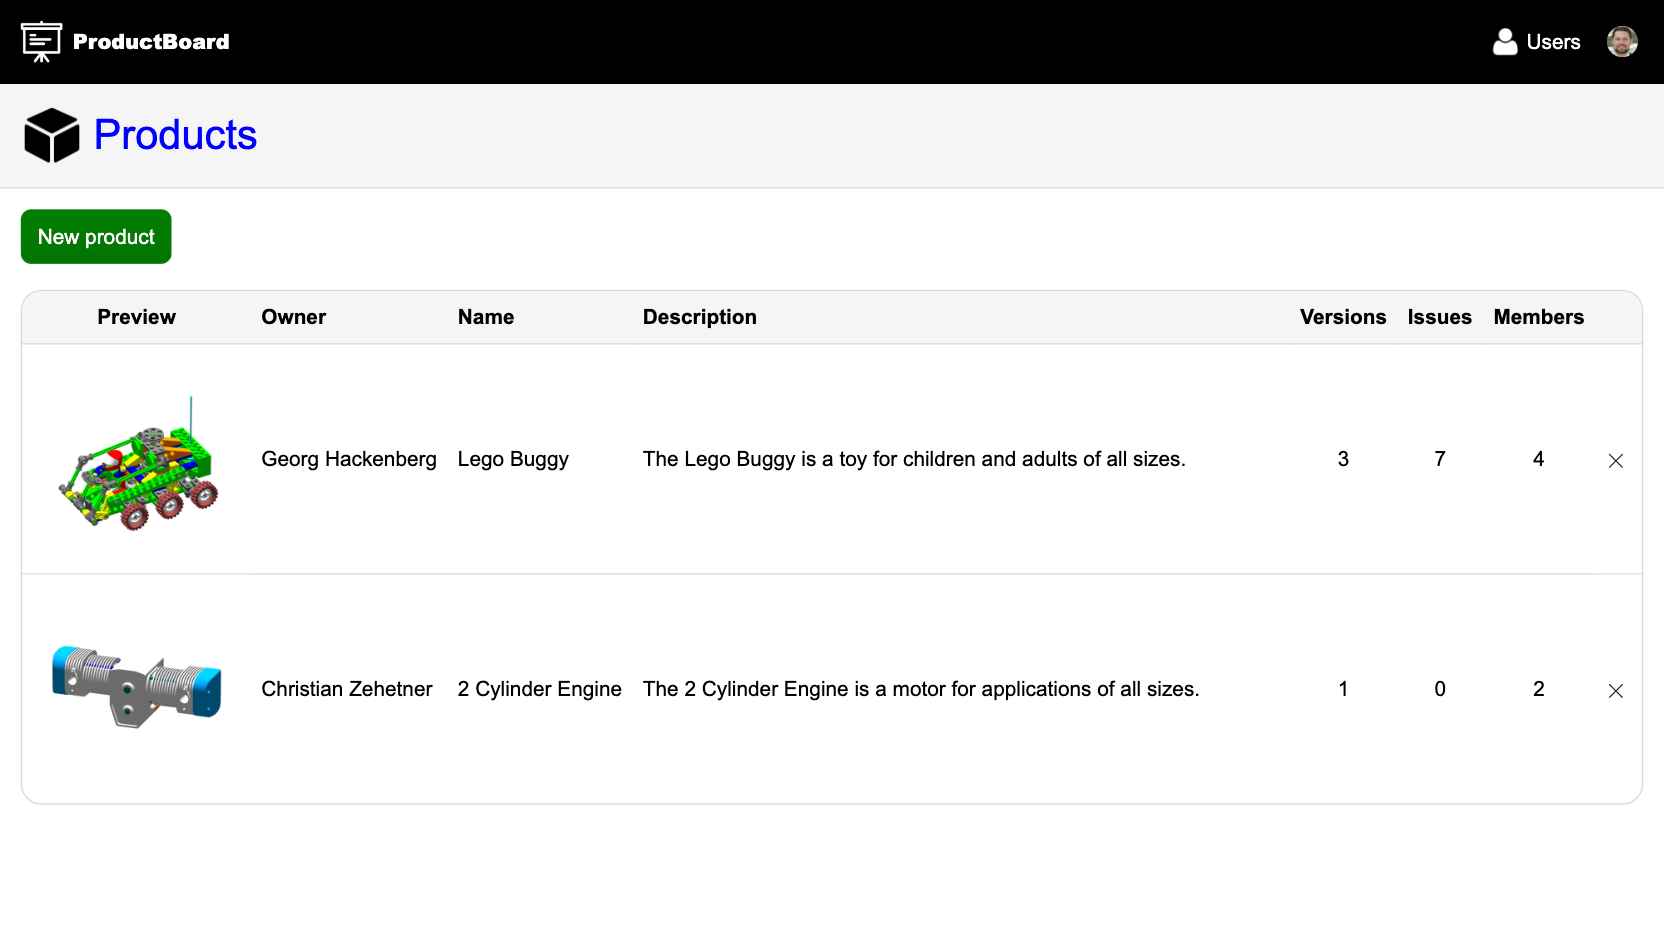
\includegraphics[width=1\textwidth]{productview.png}
    \caption{Product View}
    \label{fig: productview}
\end{figure} 

Jedes Produkt führt auf die jeweilige Produktseite, [siehe Abb. \ref{fig: versionview} auf S.~\pageref{fig: versionview}] auf der Projektmanagementtools angeboten werden, die in Tabs unterteilt sind:
\begin{itemize}
	\item Versions: In diesem Tab können über den ''New version'' Button neue Versionen hinzugefügt werden. Diese werden dann in der Listenansicht angezeigt und können durch Anklicken groß in der 3D-Ansicht auf der rechten Seite betrachtet werden.
	\item Issues: Dient zum Hinzufügen neuer Issues. Diese werden dann als Liste angezeigt und können nach offenen und geschlossenen Issues gefiltert werden. Hinter jedem Issue befindet sich ein Kommunikationskanal, wo die Issues in Textform oder durch Audioaufnahmen besprochen werden können.
	\item Milestones: Dient zum Erstellen von Sprints. Diese Sprints können dann mit Issues befüllt werden. Ein Burn-Down-Chart zeigt den Fortschritt des jeweiligen Sprints an.
	\item Members: Hier kann definiert werden, welche User der Plattform das jeweilige Produkt sehen können und welche Rechte sie haben das Produkt zu bearbeiten.
	\item Settings: Hier können der Produktname und die Produktbeschreibung nachträglich geändert werden.
\end{itemize}

\begin{figure}[h]
    \centering
    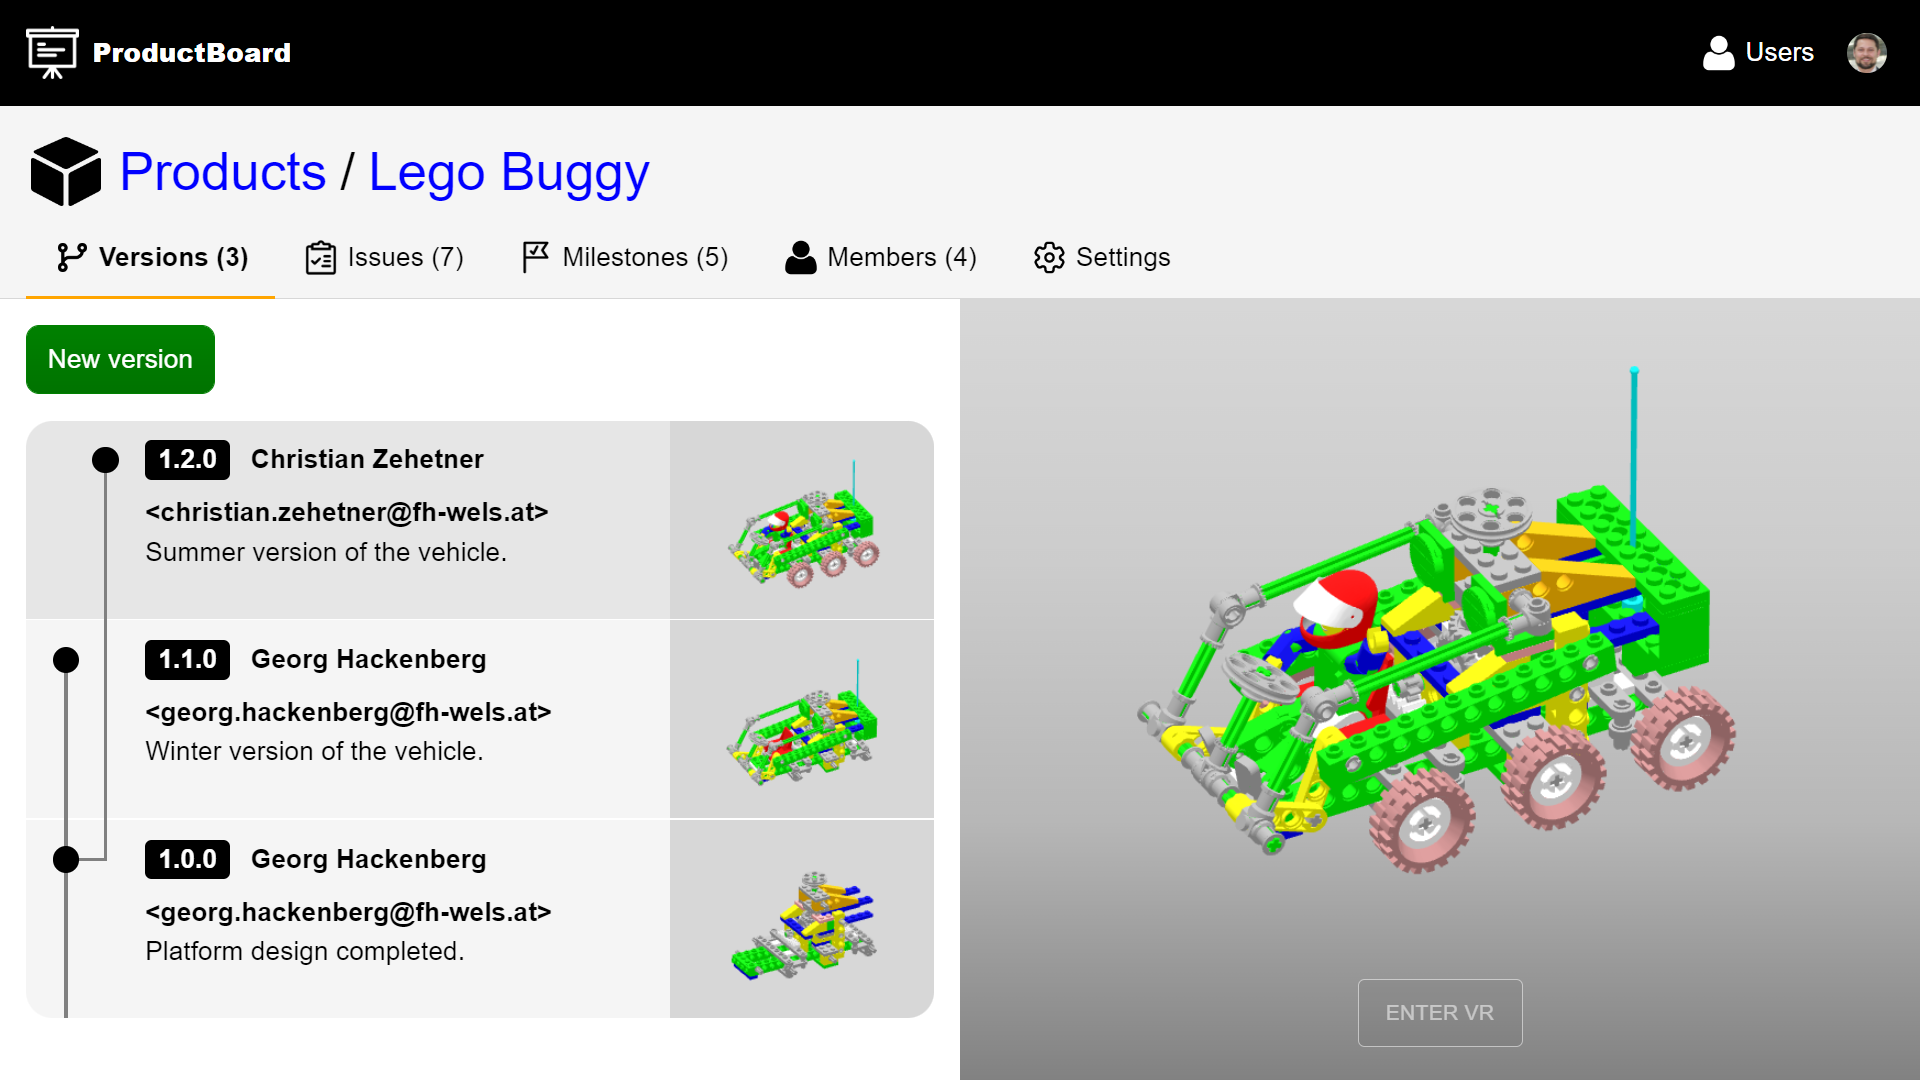
\includegraphics[width=1\textwidth]{versionview.png}
    \caption{Version View}
    \label{fig: versionview}
\end{figure}

Auf der rechten Seite wird das 3D-CAD Modell der ausgewählten Version angezeigt. Das Modell kann mit der Maus bewegt und gedreht werden. Mit dem Mausrad lässt sich die Zoomstufe einstellen. Die Applikation berücksichtigt auch kleinere Bildschirmgrößen, sodass bei kleineren Displays unten eine Tableiste erscheint, mit der zwischen der Tabellenansicht und der Modellansicht gewechselt werden kann. 